\documentclass[xcolor={dvipsnames},aspectratio=169,10pt]{beamer}
% utility packages
\usepackage{etoolbox}
\usepackage{multicol}
\usepackage{relsize}
\usepackage{fontawesome}

% better text justifying
\usepackage{microtype}
% justify text inside list environment
% Ref: http://liam0205.me/2017/04/11/justifying-in-beamer-s-lists/
\usepackage{ragged2e}
\makeatletter
\patchcmd{\itemize}{\raggedright}{\justifying}{}{}
\patchcmd{\beamer@enum@}{\raggedright}{\justifying}{}{}
\patchcmd{\@@description}{\raggedright}{\justifying}{}{}
\makeatother

% table of content with numbers and justification
% https://tex.stackexchange.com/questions/188773
\setbeamertemplate{section in toc}{\hspace*{1em}\inserttocsectionnumber.~\inserttocsection\par}
\setbeamertemplate{subsection in toc}{\hspace*{2em}\inserttocsectionnumber.\inserttocsubsectionnumber.~\inserttocsubsection\par}

% math related packages
\usepackage{amsmath}
\usepackage[ruled,vlined]{algorithm2e}
\SetAlCapNameFnt{\scriptsize}
\SetAlCapFnt{\scriptsize}
\SetAlFnt{\scriptsize}

% figure related packages
\usepackage{graphicx}
\usepackage[scale=2]{ccicons}
\usepackage{qrcode}
\usepackage{tikz}
\usepackage{tikzpagenodes}
\usetikzlibrary{positioning}

% table related packages
\usepackage{array}
\usepackage{booktabs}
\usepackage{multirow}
\usepackage{colortbl}
\newcommand{\tabincell}[2]{\begin{tabular}{@{}#1@{}}#2\end{tabular}}

% code highlight
\usepackage{listings}
\usepackage{minted}
\definecolor{mintedbg}{HTML}{E5E9F0}
\setminted{autogobble,bgcolor=mintedbg,fontsize=\small}
\setmintedinline{bgcolor=mintedbg,fontsize=\smaller}
\newminted{bash}{}
\newminted{latex}{}
\newmintinline{bash}{}
\newmintinline{latex}{}
\newcommand{\texdoc}[2]{\href{#2}{\bashinline|texdoc #1|}}

% hyperref setting
\hypersetup{
  unicode,
  psdextra,
  bookmarksnumbered=true,
  bookmarksopen=true,
  bookmarksopenlevel=3,
  bookmarksdepth=4,
  pdfcenterwindow=true,
  pdfstartview={Fit},
  pdfpagemode={FullScreen},
  pdfpagelayout={SinglePage},
}
\usepackage{bookmark}

% beamer theme
\usetheme{metropolis}
\metroset{block=fill,numbering=fraction}

% caption style
\usepackage{subcaption}
\setlength\abovecaptionskip{3pt}
\setbeamerfont{caption}{size=\scriptsize}
\renewcommand{\figurename}{Fig.}
\captionsetup{labelformat=empty,labelsep=none,textfont={bf,it}}

% Ref: https://github.com/gpoore/minted/blob/master/source/minted.dtx
\newenvironment{latexexample}
{\VerbatimEnvironment\begin{VerbatimOut}[gobble=3]{example.out}}{\end{VerbatimOut}%
  \begin{center}
    \begin{minipage}{0.47\linewidth}%
      \inputminted[resetmargins,fontsize=\scriptsize]{latex}{example.out}%
    \end{minipage}%
    \hspace{0.05\linewidth}%
    \begin{minipage}{0.47\linewidth}%
      \begin{framed}
        \setlength{\parindent}{2em}%
        \input{example.out}%
      \end{framed}
    \end{minipage}%
  \end{center}
}

\newenvironment{mathexample}
{\VerbatimEnvironment\begin{VerbatimOut}[gobble=3]{example.out}}{\end{VerbatimOut}%
  \begin{center}
    \begin{minipage}{0.47\linewidth}%
      \inputminted[resetmargins,fontsize=\scriptsize]{latex}{example.out}%
    \end{minipage}%
    \hspace{0.05\linewidth}%
    \begin{minipage}{0.47\linewidth}%
      \begin{framed}
        \[ \input{example.out} \]
      \end{framed}
    \end{minipage}%
  \end{center}
}

\newenvironment{mathexamples}
{\VerbatimEnvironment\begin{VerbatimOut}[gobble=3]{example.out}}{\end{VerbatimOut}%
  \begin{center}
    \begin{minipage}{0.47\linewidth}%
      \inputminted[resetmargins,fontsize=\scriptsize]{latex}{example.out}%
    \end{minipage}%
    \hspace{0.05\linewidth}%
    \begin{minipage}{0.47\linewidth}%
      \begin{framed}
        \directlua{
          local first = true
          for line in io.lines('example.out') do
          if first then
          first = false
          else
          tex.print('\\newline ')
          end
          tex.print('$' .. line .. '$')
          end
        }
      \end{framed}
    \end{minipage}%
  \end{center}
}


%---------------------------------------------------------------------
% Add Paper using {\paper{}. begin{beawer} ... end{beamer} }
%---------------------------------------------------------------------
\newcommand\paper[1]{
	\setbeamertemplate{footline}
	{
		\begin{beamercolorbox}[wd=\textwidth,ht=3mm,dp=03mm,leftskip=0.3cm,rightskip=0.3cm]{black}%
        		\usebeamerfont{page number in head/foot}
			(#1)\mbox{}\hfill\insertframenumber
		\end{beamercolorbox}%
	}
}
\usepackage{cite}


\title{Nonlinear analysis to quantify human movement variability from time-series data}
%\subtitle{Challenges and opportunities }
\author{ \textbf{Miguel Xochicale, PhD}  (\faTwitter @\_mxochicale \faGithub @mxochicale  )
}

\date{October 28, 2020; 17h30m BST\\
	  Neuromatch 3.0}
\institute{
	School of Biomedical Engineering and Imaging Sciences \\
	King's College London
	}

\titlegraphic{
  \begin{tikzpicture}[overlay, remember picture]
    \node[%
      above right=0.35cm and -0.2cm of current page footer area.south west,
      anchor=south west,
      inner sep=0pt] {%
      \usebeamerfont{footline}
      \begin{tabular}{lm{.8\textwidth}}
        \href{http://creativecommons.org/licenses/by/4.0/}{\ccby} &
        This work is licensed under a 
	\href{http://creativecommons.org/licenses/by/4.0/}
		{Creative Commons ``Attribution 4.0 International''} license. 
	\par Get source of this slides and see further references 
		from \url{https://github.com/mxochicale/nmc3}.
      \end{tabular}
    };
    \node[%
      above left=0.35cm and 0cm of current page footer area.south east,
      anchor=south east,
      inner sep=0pt]{\qrcode[height=1.5cm]{https://github.com/mxochicale/}};
  \end{tikzpicture}
}

\begin{document}

\maketitle

\begin{frame}{Contents}
    \tableofcontents
\end{frame}

%%%%%%%%%%%%%%%%%%%%%%%%%%%%%%%%%%%%%%%%%%%%
\section{Why Movement Variability?}


{
%\paper{
%Bernstein 1967 in \textbf{The co-ordination and regulation of movements};
%}
\begin{frame}[fragile]{Few challenges when quantifying movement variability}
  \begin{columns}
   

 \begin{column}{.3\linewidth}
    
	\textbf{Theoretical challenges}
  \begin{itemize}
        \item Modelling human movement (tasks, environments, agent, perception, action)
        \item Modelling human variability (complexity vs predictability)
        \item ?
      \end{itemize}
    \end{column}

   \begin{column}{.3\linewidth}
	
	\textbf{Choosing the right tools} 
           \begin{itemize}
                \item Time-based domain,
		\item Frequency-based domain
		\item Nonlinear dynamics
                \item ?
              \end{itemize}
	\end{column}

   \begin{column}{.3\linewidth}
	\textbf{Technical challenges}
           \begin{itemize}
                \item non-stationarity, 
		\item non-linearity, 
		\item data length, 
		\item sensor source, 
		\item noise,
                \item ?
              \end{itemize}
	\end{column}



  \end{columns}


\end{frame}
}



%%%%%%%%%%%%%%%%%%%%%%%%%%%%%%%%%%%%%%%%%%%%%%%%%%%%%%%%
{
\paper{
Bernstein 1967 in \textbf{The co-ordination and regulation of movements};
Newell and Vaillancourt 2001 in \textbf{Hum Mov Sci};
Davids et al. 2003 in \textbf{Sport Medicine};
Warren 2006 in \textbf{Psychological Review}
}
\begin{frame}{Modeling Human Movement}
    \begin{figure}
        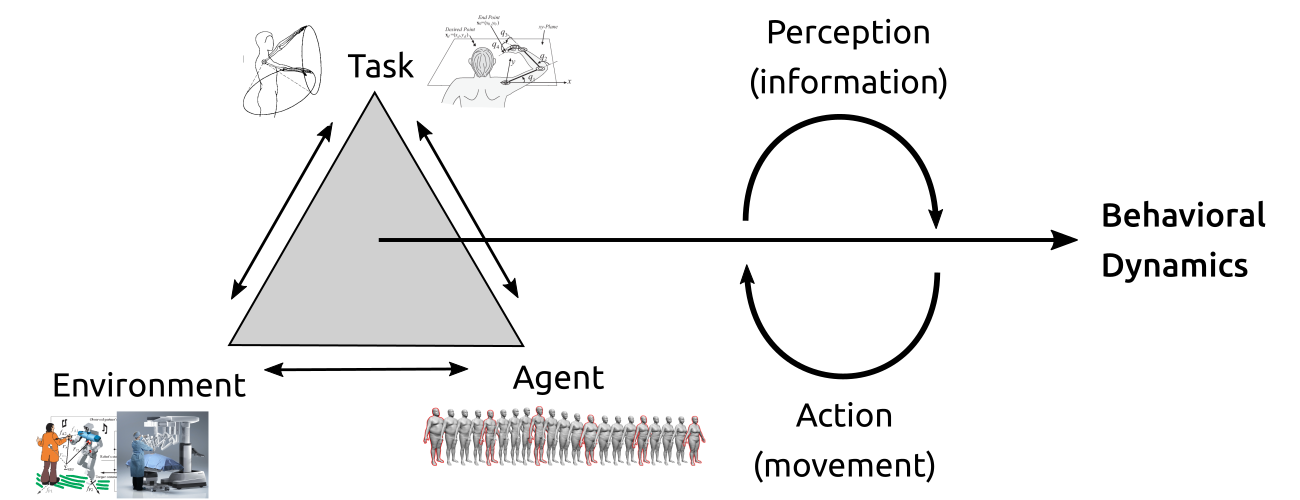
\includegraphics[width=1.0\linewidth]{./figs/modeling-movement/versions/drawing-v01.png}
	%\caption{Newell's model of movement constrains} 
   \end{figure}
\end{frame}
}



%%%%%%%%%%%%%%%%%%%%%%%%%%%%%%%%%%%%%%%%%%%%%%%%%%%%%%%%
{
\paper{
Stergiou et al. 2006 in {\bf Neurologic Physical Therapy};
Stergiou and Decker 2011 in {\bf Human Movement Science};
Tononi et al. 1998 in {\bf Trends in Cognitive Sciences}
}
\begin{frame}{Modelling Movement Variability}
    \begin{figure}
        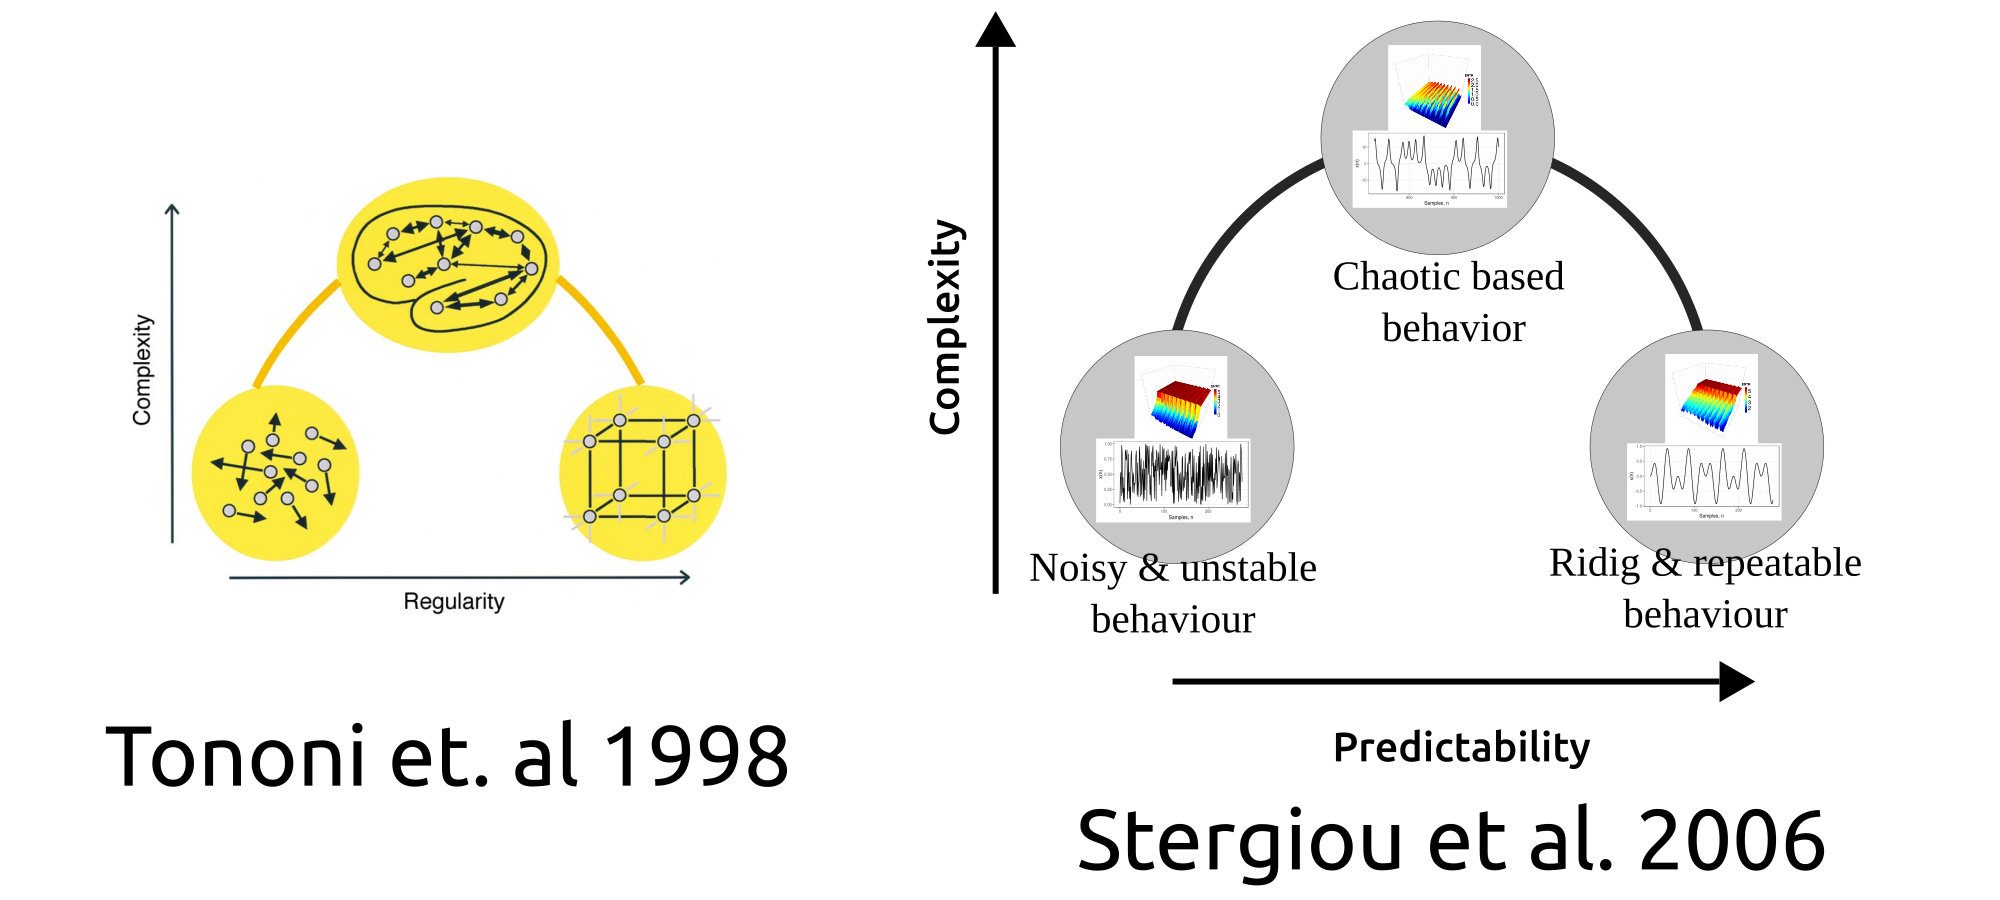
\includegraphics[width=0.95\linewidth]{./figs/modeling-movement-variability/versions/drawing-v00.png}
	%\caption{Theoretical Model of Optimal Movement Variability}
   \end{figure}
\end{frame}
}


%%%%%%%%%%%%%%%%%%%%%%%%%%%%%%%%%%%%%%%%%%%%
\section{Nonlinear Methods}

{
\paper{\textbf{M. Xochicale 2019} PhD thesis, DOI:10.5281/zenodo.3384145}
\begin{frame}{Nonlinear Analysis}
    \vspace{-00mm}
      \begin{figure}
        \centering
        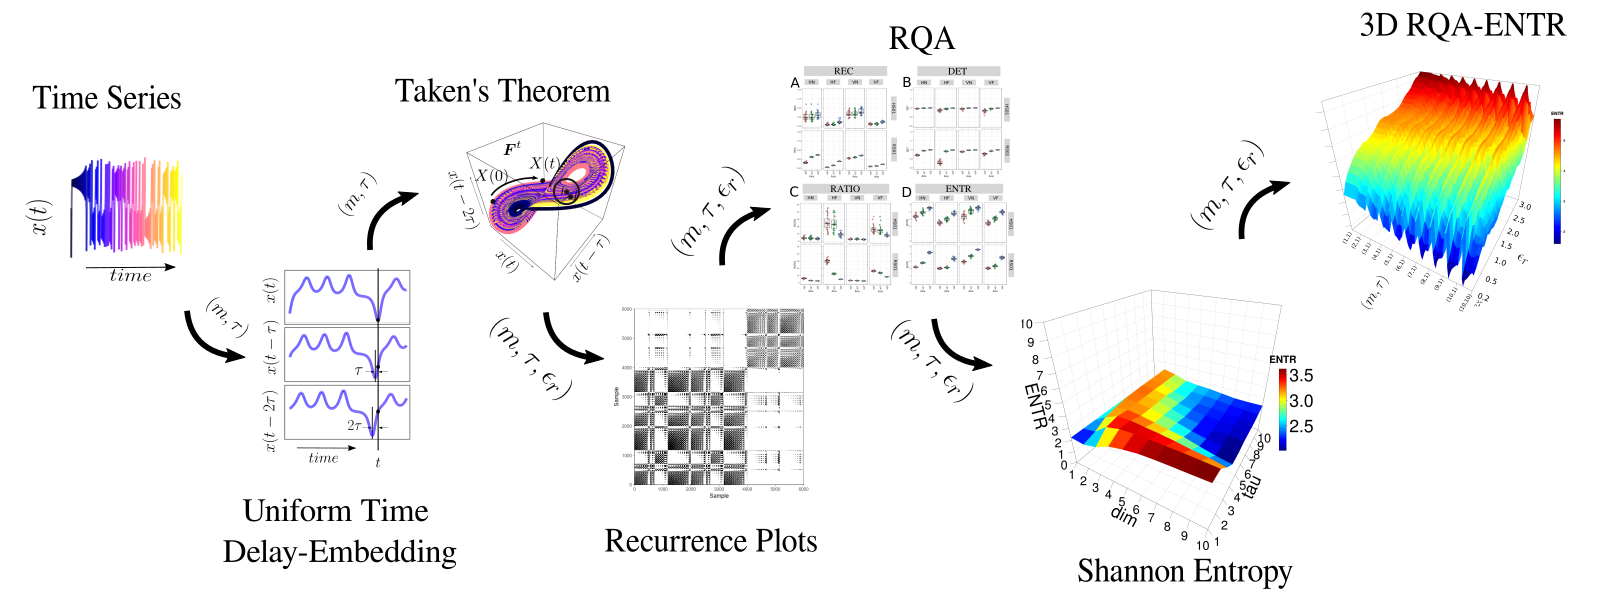
\includegraphics[width=0.99\linewidth]{./figs/nonlinear-methods/versions/drawing-v00.png}
        \caption{}
      \end{figure}
\end{frame}
}



%\subsection{References}
%%%%%%%%%%%%%%%%%%%%%%%%%%%%%%%%%%%%%%%%%%%%%%%%%%%%%%%%
\begin{frame}{References}
    \begin{thebibliography}{10}

\beamertemplatearticlebibitems

	\bibitem{xochicale2020}
	Xochicale Miguel
	\newblock 
	Nonlinear methods to quantify Movement Variability 
	in Human-Humanoid Interaction Activities
	\newblock In Submission to Scientific Reports  
      	\newblock \url{https://arxiv.org/abs/1810.09249}

	%\bibitem{xochicale2019}
	%Xochicale Miguel
	%\newblock 
	%Nonlinear Analysis to Quantify Movement 
	%Variability in Human-Humanoid Interaction 
      	%\newblock Open Access Ph.D. Thesis (2019) 
      	%\newblock \url{https://github.com/mxochicale-phd/thesis}

    \end{thebibliography}
\end{frame}



\begin{frame}[standout]
  Thanks \\
  Questions?
\end{frame}

\end{document}
